
\section{Classifying OpenMP workshares}

The parallelism in an OpenMP application program is expressed through
parallel regions, worksharing constructs, and combined parallel
constructs. A combined parallel construct can be considered as a
parallel region with only one worksharing construct inside it,
although its implementation may be more efficient from a performance
point of view. In any case, a parallel region is the basic concept
in OpenMP programming.

When a parallel region starts, multiple threads will execute the code
inside the region concurrently\cite{Cha01}.

\begin{figure}[!h]
  \begin{center}
    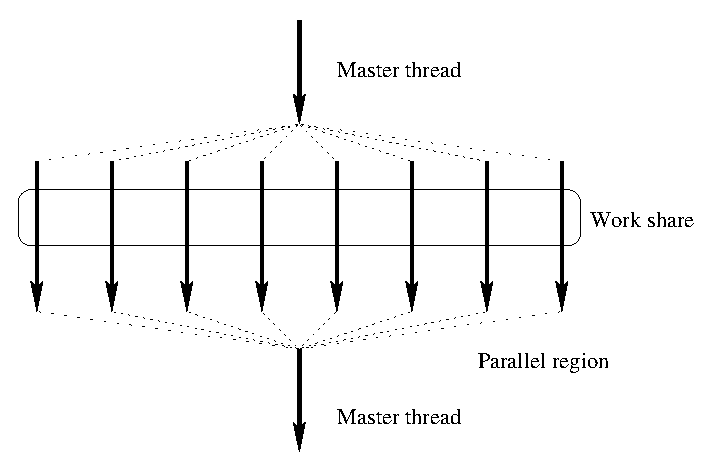
\includegraphics[angle=0, width=0.65\textwidth]{parregion.eps}
    \caption{\footnotesize Parallel region}
    \label{fig:parregion}
  \end{center}
\end{figure}

In Figure \ref{fig:parregion}, a master thread starts up a parallel
region executed by 8 threads. Through parallel regions, multiple
threads accomplish \emph{worksharing} in an OpenMP program.

The simplest format of worksharing is replicated execution of the same
code segment on different threads. It is more useful to divide work
among multiple threads --- either by having different threads operate
on different portions of a shared data structure, or by having
different threads perform entirely different tasks. Each cooperation of this
kind is considered as a \emph{workshare}\footnote{The
  concept of workshare here is different from the parallel construct,
  \texttt{WORKSHARE} in Fortran OpenMP specification 2.0, which can be
  treated semantically as the combination of \texttt{OMP DO} and
  \texttt{OMP SINGLE} constructs.} in this paper. In the figure, we
use a round-cornered rectangular block to represent one workshare.

The most common forms of workshares in OpenMP specification are
worksharing DO and SECTIONS, as shown in Figure \ref{fig:workshare} (a)
and (b) respectively.

\begin{figure}[!h]
  \begin{center}
    \includegraphics[angle=0, width=0.6\textwidth]{workshare.eps}
    \caption{\footnotesize Common workshare}
    \label{fig:workshare}
  \end{center}
\end{figure}

We use different numbers to mark the sequential order of the blocks in
an OpenMP DO construct, but it does not mean the implementation will
ensure that the corresponding threads will work on those blocks. In
fact, the mapping of work to threads is determined by the schedule
type of the DO construct as specified by the OpenMP standard. Similarly,
the mapping between the sections in a SECTIONS construct and the
threads is also decided by the schedule type.  The fundamental
difference between a DO construct and a SECTIONS construct is that in
SECTIONS the code segments executed by threads could be entirely
different.

Besides the common workshares introduced above, we can consider
other OpenMP structures as workshares too. The typical examples are
SINGLE constructs and explicit barriers, as in Figure
\ref{fig:synchronization} (a) and (b).

\begin{figure}[!h]
  \begin{center}
    \includegraphics[angle=0, width=0.6\textwidth]{synchronization.eps}
    \caption{\footnotesize Synchronization workshare}
    \label{fig:synchronization}
  \end{center}
\end{figure}

A SINGLE construct is semantically equivalent to a SECTIONS construct
with only one SECTION inside, while the explicit barrier is like a
SECTIONS construct with neither NOWAIT clauses nor any SECTION inside.
For a SINGLE construct, the first thread that encounters the code will
execute the block. This is different from a MASTER construct, where
the decision can be made simply by checking the thread ID.

Worksharing DO, SECTIONS and SINGLE constructs have an important common
feature: they have an implicit barrier at the end of the construct,
which may be disabled by using the optional NOWAIT clause. An explicit
BARRIER is semantically equivalent to an empty SINGLE section without
the NOWAIT clause. This observation leads us to classify explicit
barriers in the same category of workshare constructs.

Different implementations may have a different view of this kind of
classification. The real advantage of considering them all as
workshares is for practical coding. From an implementation point of
view, their common behaviors will lead to a common code base, thus
improving the overall code quality.

From now on, we will use \emph{workshare} to refer to any one of the
workshares we have mentioned above.

